\chapter{Evaluation of playing strenght}\label{cap:analysis}

This chapter documents the implementation of the following techniques used to improve the chess engine:

\begin{itemize}[itemsep=1pt]
    \item Transposition tables with zobrist hashing.
    \item Move generator with magic bitboards and PEXT instructions.
    \item Evaluation with king safety and piece mobility parameters.
    \item Multithread search.
    \item Search with Late move Reductions.
\end{itemize}

All of these improvements have been compared with each other using \textit{CuteChess}, and the best version was also evaluated against \textit{Stockfish}. These comparisons were conducted on machines provided by GitHub Actions.

\section{GitHub Actions and Workflows}

GitHub Actions is a CI/CD tool integrated into GitHub that allows developers to automate tasks such as building, testing, and deploying code. Workflows are defined in YAML files and specify the tasks to be executed, the jobs or events that trigger them, and the environment in which they run.

\vspace{1em}

\noindent In this project, since it is public in a GitHub repository, we used GitHub Actions to automate the testing and evaluation of the chess engine with \textit{Stockfish} and \textit{CuteChess}. A workflow was configured (located at \texttt{.github\textbackslash{}workflows\textbackslash{}manual-workflow.yml}) to compile the engine and run automated games using \textit{CuteChess} between different versions of the engine or against \textit{Stockfish}.

\vspace{1em}

\noindent At the end of each section, we provide the results of a 100-game match between the improved engine and a baseline version. The baseline includes only the core techniques discussed in the previous chapter on engine architecture. The purpose of these matches is to measure the improvement in playing strength introduced by each new implementation.

\vspace{1em}

\noindent All matches are conducted using the tournament manager \textit{CuteChess}~\cite{CuteChess} with the following configuration:

\begin{itemize}[itemsep=1pt]
\item 100 games per match.
\item 50 unique random starting positions, each played twice with alternating colors.
\item 4 seconds of thinking time per move.
\item A 150-move limit per game, after which the game is declared a draw.
\end{itemize}

\noindent The matches were executed on virtual machines provided by GitHub Actions, using the \texttt{ubuntu-latest} runner. At the time of testing, this environment provided 4 CPUs, 16~GB of RAM, a 14~GB SSD, and a 64-bit architecture.

\section{Transposition Table}\label{sec:tt}

\subsection{Analysis}

\noindent To evaluate the impact of introducing the transposition table, we conducted the 100-game tournament against the baseline version of the engine. The~\cref{tab:tt_vs_basic} details the implementation used for each bot.

\vspace{1em}

\begin{table}
    \centering
    \begin{tabular}{|p{4cm}|p{4cm}|p{4cm}|}
    \hline
    \textit{Component}         & \textit{Transposition Table Bot}  & \textit{Basic Bot}     \\ \hline
    Search                     & Alpha-beta With Transposition Table          & Basic Alpha-beta           \\ \hline
    Evaluation Function        & Materialistic                      & Materialistic       \\ \hline
    Move Generator             & Basic implementation              & Basic implementation   \\ \hline
    Move Ordering              & MVV-LVA                           & MVV-LVA                \\ \hline
    \end{tabular}
    \caption{Match configuration: Transposition Table Bot vs Basic Bot}\label{tab:tt_vs_basic}
\end{table}

\noindent As illustrated in following result bar, we see a substantial improvement by adding the transposition table with 46 wins versus 32 losses. The remaining 22 games ended in a draw.

\begin{center}
\ResultBar{15cm}{0.5cm}{46}{22}{32}
\medskip
\end{center}

\section{Move generator with Magic Bitboards and PEXT instructions}

\subsection{Analysis}

\noindent To evaluate the impact of introducing the move generator accelerated with PEXT instructions, we conducted the 100-game tournament against the baseline version of the engine. The~\cref{tab:pext_vs_basic} details the implementation used for each bot.

\vspace{1em}

\begin{table}
    \centering
    \begin{tabular}{|p{4cm}|p{4cm}|p{4cm}|}
    \hline
    \textit{Component}         & \textit{PEXT instructions Bot}  & \textit{Basic Bot}     \\ \hline
    Search                     & Alpha-beta With Transposition Table          & Basic Alpha-beta           \\ \hline
    Evaluation Function        & Materialistic                      & Materialistic       \\ \hline
    Move Generator             & PEXT implementation              & Basic implementation   \\ \hline
    Move Ordering              & MVV-LVA                           & MVV-LVA                \\ \hline
    \end{tabular}
    \caption{Match configuration: PEXT instructions Bot vs Basic Bot}\label{tab:pext_vs_basic}
\end{table}

\noindent As illustrated in the following result bar, we achieved a significant performance improvement by adding the PEXT instructions with 46 wins versus 22 losses. The remaining 14 games ended in a draw.

\begin{center}
\ResultBar{15cm}{0.5cm}{64}{14}{22}
\medskip
\end{center}

\section{Evaluation with King Safety and piece mobility}

\subsection{Analysis}

To evaluate the impact of introducing the new parameters in the evaluation, we conducted the 100-game tournament against the baseline version of the engine. The~\cref{tab:safety_mobility_vs_basic} details the implementation used for each bot.

\vspace{1em}

\begin{table}
    \centering
    \begin{tabular}{|p{4cm}|p{4cm}|p{4cm}|}
    \hline
    \textit{Component}         & \textit{PEXT instructions Bot}  & \textit{Basic Bot}     \\ \hline
    Search                     & Alpha-beta With Transposition Table          & Basic Alpha-beta           \\ \hline
    Evaluation Function        & Safety and Mobility                      & Materialistic      \\ \hline
    Move Generator             & PEXT implementation              & Basic implementation   \\ \hline
    Move Ordering              & MVV-LVA                           & MVV-LVA                \\ \hline
    \end{tabular}
    \caption{Match configuration: King Safety and Piece mobility eval Bot vs Basic Bot}\label{tab:safety_mobility_vs_basic}
\end{table}

\noindent As illustrated in the following result bar, the results are slightly worse compared to the match using the material-only evaluation shown in the following result bar, with 62 wins and 30 losses. This decline may be attributed to the additional computational overhead introduced by evaluating the new parameters. Moreover, while concepts such as king safety and piece mobility are intuitively valuable to human players, the engine may struggle to consistently associate them with actual positional strength.

\begin{center}
\ResultBar{15cm}{0.5cm}{62}{8}{30}
\medskip
\end{center}

\section{Multithreaded Search}

\subsection{Analysis}

To evaluate the improvement in the new evaluation, we conducted the same 100 game match vs the basic bot version. 

\begin{center}
\ResultBar{15cm}{0.5cm}{32}{5}{63}
\medskip
\end{center}

\noindent The results are slightly worse compared to the match using the material-only evaluation, with 8 more losses than before. This may be due to the increased computational cost of evaluating these additional parameters. Furthermore, although these are abstract concepts commonly used by humans to assess positions, the engine may struggle to find a clear correlation between them and actual positional strength.

\section{Late Move Reductions}

We experiment with the use of late move pruning, under the assumption that if our move ordering is good, the best move in the position should be among the first explored moves. We reduce the depth by one unit starting from the tenth movement.

\subsection*{Analysis}

To evaluate the improvement in the new evaluation, we conducted the same 100 game match vs the basic bot version.

\begin{center}
 \ResultBar{15cm}{0.5cm}{48}{15}{37}
\medskip
\end{center}

\noindent The results are worse, with 15 more losses than the version without this aggresive pruning. This could be because our move ordering is not that strong, and the best move in the position sometimes is in the last positions.

\section{Engine Final Evaluation}

\noindent Figure~\cref{fig:eloDistribution} shows the Elo rating distribution of players on Lichess as of May 2025, where the median rating is approximately 1500.

\vspace{1em}

\noindent AlphaDeepChess has achieved a rating of 1900 on Lichess~\cite{AlphaDeepChessElo}, placing it well above the median and within the top percentiles of the player base. For comparison, the highest-rated human player on the platform has a rating of 3003, while the chess engine Stockfish has been benchmarked at approximately 3644 Elo~\cite{StockfishElo}.

\begin{figure}[h]
    \centering
    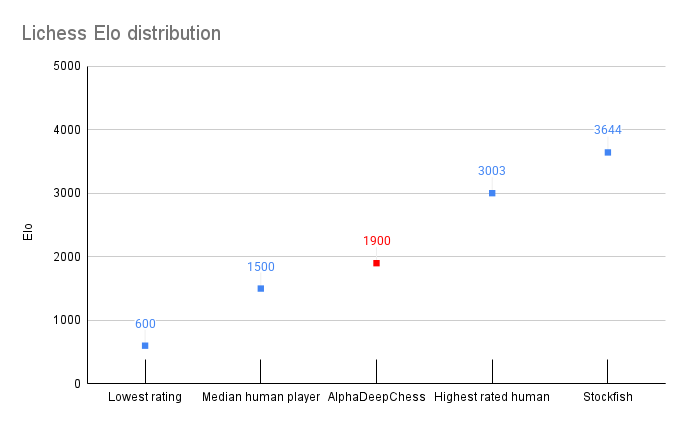
\includegraphics[width=0.95\linewidth]{Imagenes/eloDistribution.png}
    \caption{Lichess Elo distribution~\cite{LichessEloDistribution}.}
    \label{fig:eloDistribution}
\end{figure}